\documentclass[dvipdfmx,a4paper,11pt]{article}
\usepackage[utf8]{inputenc}
%\usepackage[dvipdfmx]{hyperref} %リンクを有効にする
\usepackage{url} %同上
\usepackage{amsmath,amssymb} %もちろん
\usepackage{amsfonts,amsthm,mathtools} %もちろん
\usepackage{braket,physics} %あると便利なやつ
\usepackage{bm} %ラプラシアンで使った
\usepackage[top=30truemm,bottom=30truemm,left=25truemm,right=25truemm]{geometry} %余白設定
\usepackage{latexsym} %ごくたまに必要になる
\renewcommand{\kanjifamilydefault}{\gtdefault}
\usepackage{otf} %宗教上の理由でmin10が嫌いなので


\usepackage[all]{xy}
\usepackage{amsthm,amsmath,amssymb,comment}
\usepackage{amsmath}    % \UTF{00E6}\UTF{0095}°\UTF{00E5}\UTF{00AD}\UTF{00A6}\UTF{00E7}\UTF{0094}¨
\usepackage{amssymb}  
\usepackage{color}
\usepackage{amscd}
\usepackage{amsthm}  
\usepackage{wrapfig}
\usepackage{comment}	
\usepackage{graphicx}
\usepackage{setspace}
\setstretch{1.2}


\newcommand{\R}{\mathbb{R}}
\newcommand{\Z}{\mathbb{Z}}
\newcommand{\Q}{\mathbb{Q}} 
\newcommand{\N}{\mathbb{N}}
\newcommand{\C}{\mathbb{C}} 
\newcommand{\Sin}{\text{Sin}^{-1}} 
\newcommand{\Cos}{\text{Cos}^{-1}} 
\newcommand{\Tan}{\text{Tan}^{-1}} 
\newcommand{\invsin}{\text{Sin}^{-1}} 
\newcommand{\invcos}{\text{Cos}^{-1}} 
\newcommand{\invtan}{\text{Tan}^{-1}} 
\newcommand{\Area}{\text{Area}}
\newcommand{\vol}{\text{Vol}}




   %当然のようにやる.
\allowdisplaybreaks[4]
   %もちろん.
%\title{第1回. 多変数の連続写像 (岩井雅崇, 2020/10/06)}
%\author{岩井雅崇}
%\date{2020/10/06}
%ここまで今回の記事関係ない
\usepackage{tcolorbox}
\tcbuselibrary{breakable, skins, theorems}

\theoremstyle{definition}
\newtheorem{thm}{定理}
\newtheorem{lem}[thm]{補題}
\newtheorem{prop}[thm]{命題}
\newtheorem{cor}[thm]{系}
\newtheorem{claim}[thm]{主張}
\newtheorem{dfn}[thm]{定義}
\newtheorem{rem}[thm]{注意}
\newtheorem{exa}[thm]{例}
\newtheorem{conj}[thm]{予想}
\newtheorem{prob}[thm]{問題}
\newtheorem{rema}[thm]{補足}

\DeclareMathOperator{\Ric}{Ric}
\DeclareMathOperator{\Vol}{Vol}
 \newcommand{\pdrv}[2]{\frac{\partial #1}{\partial #2}}
 \newcommand{\drv}[2]{\frac{d #1}{d#2}}
  \newcommand{\ppdrv}[3]{\frac{\partial #1}{\partial #2 \partial #3}}



%ここから本文.
\begin{document}
%\maketitle
\begin{center}
{ \large 大阪市立大学 R3年度(2021年度)前期 全学共通科目 解析 I *TI電(都1\UTF{FF5E}28)} \\
\vspace{5pt}

{\LARGE 中間レポート解答例} \\
\vspace{5pt}

%{ \Large 提出締め切り 2021年6月8日 23時59分00秒 (日本標準時刻)}
\end{center}

\begin{flushright}
 担当教官: 岩井雅崇(いわいまさたか) 
\end{flushright}

{\Large 第1問.} (授業第6回の内容.)
\vspace{11pt}

次の(1)から(4)までの関数について, $x=0$の近くでの漸近展開を3次まで求めよ.


\vspace{11pt}

(1). $\sqrt{x+1}$\,\,\,
(2). $\Tan x$ \,\,\,
(3). $\cosh x$ \,\,\,
(4). $(1+ x) \sin x$
%(4). $\frac{x}{1-e^{-x}}$
%\begin{enumerate}\item[問1.] $\sqrt{x}$\item[問2.] $\Tan x$\item[問3.] $\cosh x$\item[問4.] $\frac{x}{1-e^{-x}}$\end{enumerate}

\vspace{11pt}

\underline{ただし答えを導出する過程を記した上で, 答えは次のように書くこと.}

\vspace{11pt}

(例題1) $e^x$ 

(答え) $e^x = 1 + x + \frac{x^2}{2} + \frac{x^3}{6}  + o(x^3)$\,\,\,
$(x \rightarrow 0)$


\vspace{11pt}

(例題2) $\cos x$

(答え) $\cos x= 1 - \frac{x^2}{2} + o(x^3)$\,\,\,$(x \rightarrow 0)$

 \vspace{11pt}
 
\hspace{-11pt}{\Large $\bullet$ 第1問解答例.}

$C^{\infty}$関数$f(x)$に関して
 $$f(x) = f(0) + f'(0) x+ \frac{f''(0)}{2} x + \frac{f'''(0)}{6} x^3 +
 o(x^3)\,\,\,
(x \rightarrow 0) \text{である.}$$

 
 (1). $f(x)=\sqrt{x+1} = (x+1)^{\frac{1}{2}}$とおくと, 
   \begin{align*}
\begin{split}
f(x) = (x+1)^{\frac{1}{2}} \text{\,\,\, より\,\,}& f(0)=1\\
f'(x) = \frac{1}{2}(x+1)^{-\frac{1}{2}} \text{\,\,\, より\,\,}& f'(0)=\frac{1}{2}\\
f''(x) = -\frac{1}{4}(x+1)^{-\frac{3}{2}} \text{\,\,\, より\,\,}& f''(0)=-\frac{1}{4}\\
f'''(x) = \frac{3}{8}(x+1)^{-\frac{5}{2}} \text{\,\,\, より\,\,}& f'''(0)=\frac{3}{8}\\
\end{split}
\end{align*}

 $$
 \text{よって}
\sqrt{x+1} = 1+\frac{1}{2}x -\frac{1}{8}x^2 +\frac{1}{16}x^3 + o(x^3)\,\,\,
(x \rightarrow 0) \text{である.}
 $$
 
  (2). $f(x)=\Tan x$とおくと, 
   \begin{align*}
\begin{split}
f(x) = \Tan x \text{\,\,\, より\,\,}& f(0)=0\\
f'(x) = (x^2+1)^{-1} \text{\,\,\, より\,\,}& f'(0)=1\\
f''(x) = -2x(x^2+1)^{-2}\text{\,\,\, より\,\,}& f''(0)=0\\
f'''(x) = 8x^2(x^2+1)^{-3} -2(x^2+1)^{-2} \text{\,\,\, より\,\,}& f'''(0)=-2\\
\end{split}
\end{align*}
 $$
  \text{よって}
\Tan x= x -\frac{1}{3}x^3 + o(x^3)\,\,\,
(x \rightarrow 0) \text{である.}
 $$
 
   (3). $f(x)=\cosh x = \frac{e^x + e^{-x}}{2}$とおくと, 
   \begin{align*}
\begin{split}
f(x) = \sinh x \text{\,\,\, より\,\,}& f(0)=1\\
f'(x) = \cosh x \text{\,\,\, より\,\,}& f'(0)=0\\
f''(x) = \sinh x\text{\,\,\, より\,\,}& f''(0)=1\\
f'''(x) = \cosh x \text{\,\,\, より\,\,}& f'''(0)=0\\
\end{split}
\end{align*}
 $$
 \text{よって}
\cosh x= 1 + \frac{1}{2}x^2 + o(x^3)\,\,\,(x \rightarrow 0) \text{である.}
 $$
 
 [別解].
$$
e^x = 1+ x + \frac{1}{2}x^2 + \frac{1}{6}x^3 +o(x^3)\,\,\, (x \rightarrow 0) 
$$
$$
e^{-x} = 1- x + \frac{1}{2}x^2 - \frac{1}{6}x^3 +o(x^3)\,\,\, (x \rightarrow 0) 
$$
であるため, 
  \begin{align*}
\begin{split}
\cosh x = \frac{e^x + e^{-x}}{2}
&=\frac{1}{2}\left(1+ x + \frac{1}{2}x^2 + \frac{1}{6}x^3\right)+\frac{1}{2}\left(1- x + \frac{1}{2}x^2 - \frac{1}{6}x^3 \right) + o(x^3)\,\,\, (x \rightarrow 0)  \\
&=1 + \frac{1}{2}x^2 + o(x^3)\,\,\,(x \rightarrow 0) \text{である.}
\end{split}
\end{align*}

  (4). $f(x)=(1+x)\sin x $とおくと, 
   \begin{align*}
\begin{split}
f(x) = (1+x)\sin x  \text{\,\,\, より\,\,}& f(0)=0\\
f'(x) = \sin x + (1+x)\cos x \text{\,\,\, より\,\,}& f'(0)=1\\
f''(x) = 2 \cos x -(1+x)\sin x \text{\,\,\, より\,\,}& f''(0)=2\\
f'''(x) = -3 \sin x-(1+x)\cos x \text{\,\,\, より\,\,}& f'''(0)=-1\\
\end{split}
\end{align*}

 $$
 \text{よって}
(1+x)\sin x = x + x^2 -  \frac{1}{6}x^3 + o(x^3)\,\,\,(x \rightarrow 0) \text{である.}
 $$

 [別解].
$$
\sin x  = x -  \frac{1}{6}x^3 +o(x^3)\,\,\, (x \rightarrow 0) \text{より, }
x \sin x = x^2  +o(x^3)\,\,\, (x \rightarrow 0) \text{であるので, }
$$
 $$
(1+x)\sin x = x + x^2 -  \frac{1}{6}x^3 + o(x^3)\,\,\,(x \rightarrow 0) \text{である.}
 $$


  \vspace{33pt}
      
 {\Large 第2問.} (授業第5回の内容.)
 \vspace{11pt}
 
(1).
$[0, \frac{\pi}{2}]$上で次の不等式が成り立つことを示せ.
$$
x - \frac{x^3}{3!} + \frac{x^5}{5!} - \frac{x^7}{7!}
\leqq \sin x
\leqq  
x - \frac{x^3}{3!} + \frac{x^5}{5!}
$$

\vspace{11pt}

(2).
$\sin 1$を小数第3位まで求めよ.

 \vspace{11pt}
 
\hspace{-11pt}{\Large $\bullet$ 第2問解答例.}

(1). 有限テイラー展開の定理より, 任意の$x \in [0, \frac{\pi}{2}]$について, ある$\theta \in (0,1)$があって
$$
\sin x = x - \frac{x^3}{3!} + \frac{x^5}{5!} -\frac{\sin(\theta x)}{6!}x^6
$$
 となる.
 $\theta x \in [0, \frac{\pi}{2}]$から, $-\frac{\sin(\theta x)}{6!}x^6 \leqq 0$であるので, 
$$
\sin x = x - \frac{x^3}{3!} + \frac{x^5}{5!} -\frac{\sin(\theta x)}{6!}x^6
\leqq x - \frac{x^3}{3!} + \frac{x^5}{5!}\text{である.}
$$ 

同様に任意の$x \in [0, \frac{\pi}{2}]$について, ある$\theta \in (0,1)$があって
$$
\sin x = x - \frac{x^3}{3!} + \frac{x^5}{5!} - \frac{x^7}{7!} + \frac{\sin(\theta x)}{8!}x^8
$$
 となる.
 $\theta x \in [0, \frac{\pi}{2}]$から, $\frac{\sin(\theta x)}{8!}x^8\geqq 0$であるので, 
$$
\sin x = x - \frac{x^3}{3!} + \frac{x^5}{5!} - \frac{x^7}{7!} + \frac{\sin(\theta x)}{8!}x^8
\geqq x - \frac{x^3}{3!} + \frac{x^5}{5!} - \frac{x^7}{7!} \text{である.}
$$ 

 [補足]. 普通に微分を5回(または7回)やって増減表を書いて示すこともできます. 

(2). $0 <1 < \frac{\pi}{2}$より, (1)の不等式に$x=1$を代入して, 
$$
1 - \frac{1}{3!} + \frac{1}{5!} - \frac{1}{7!}
\leqq \sin 1
\leqq  
1 - \frac{1}{3!} + \frac{1}{5!} \text{である.}
$$
$$
1 - \frac{1}{3!} + \frac{1}{5!} - \frac{1}{7!} =\frac{4241}{5040} = 0.8414\cdots \geqq0.8414, 
1 - \frac{1}{3!} + \frac{1}{5!}  =\frac{101}{120} = 0.84166\cdots \leqq 0.84167 \text{より, }
$$
$
0.8414 \leqq \sin 1 \leqq 0.84167
$
であるので, $\sin 1$の小数第3位までの値は0.841である.
   \vspace{33pt}
   
   {\Large 第3問.} (授業第3回の内容.)
    \vspace{11pt}
 
 $\theta = \Tan \left( \frac{1}{5} \right)$とおく.
 次の問いに答えよ.
 
 \vspace{11pt}
 
(1).  $\tan(2 \theta)$の値を求めよ.

    \vspace{11pt}
    
(2).  $\tan(4 \theta)$の値を求めよ.

\vspace{11pt}

(3).  $\tan(4 \theta - \frac{\pi}{4})$の値を求めよ.

\vspace{11pt}

(4).  次の式を示せ.
$$
\frac{\pi}{4} = 4 \, \Tan \left(\frac{1}{5} \right)-  \Tan \left( \frac{1}{239} \right)
$$
 \vspace{11pt}
 
\hspace{-11pt}{\Large $\bullet$ 第3問解答例.}

解答の前に加法定理を思い出しておく.
$$
\tan (x+y) = \frac{\tan x + \tan y}{1 - \tan x \tan y } \,\,\,
\tan (x-y) = \frac{\tan x - \tan y}{1 +\tan x \tan y }
$$

(1).
$$
\tan(2 \theta) = \frac{2 \tan \theta}{1 - (\tan \theta)^2}
=\frac{\frac{2}{5}}{1 - \frac{1}{25}} = \frac{5}{12}
$$

(2).
$$
\tan(4 \theta) = \frac{2 \tan 2\theta}{1 - (\tan 2\theta)^2}
=\frac{\frac{10}{12}}{1 - \frac{25}{144}} = \frac{120}{119}
$$

(3).
$$
\tan(4 \theta - \frac{\pi}{4}) = \frac{\tan 4\theta - \tan \frac{\pi}{4} }{1 + (\tan 4\theta )(\tan \frac{\pi}{4}) }
=\frac{\frac{120}{119} -1 }{1 + \frac{120}{119}} = \frac{1}{239}
$$

(4). (3)から
$$
\Tan \left(\frac{1}{239} \right) = 4 \theta - \frac{\pi}{4} = 4 \, \Tan \left( \frac{1}{5} \right) - \frac{\pi}{4} 
$$
であるので, 
$$
\frac{\pi}{4} = 4 \, \Tan \left(\frac{1}{5} \right)-  \Tan \left( \frac{1}{239} \right)
\text{\,となる.}
$$

     \vspace{33pt} 
     
   
{\Large 第4問.} (授業第4回の内容.)
    \vspace{11pt}

 $
 f(x) = \frac{x^3 -1 }{2}
 $
 とおく. 次の問いに答えよ.
 
 \vspace{11pt}
 
 (1). $f(x)$は$\R$上で単調増加であることを示せ.
 
 \vspace{11pt}
 
 (2). 方程式$ \sqrt[3]{2x + 1} = \frac{x^3 - 1}{2}$の実数解を全て求めよ.
 
  \vspace{11pt}
 
\hspace{-11pt}{\Large $\bullet$ 第4問解答例.}

(1). $f'(x) = \frac{3}{2}x^2$である. 
$(- \infty , 0)$上で$f'(x)>0$であるので, $f(x)$は$(-\infty, 0]$上で単調増加である.
また$(0, +\infty)$上で$f'(x)>0$であるので, $f(x)$は$[0, +\infty)$上で単調増加である.
よって$f(x)$は$\R$上で単調増加である.

(2). 解答は2通りあります.

[解答1]. $\alpha$を方程式$ \sqrt[3]{2x + 1} = \frac{x^3 - 1}{2}$の実数解とし, $\beta = f(\alpha)$とする.
$f(\alpha) = \frac{\alpha^3 -1}{2} = \sqrt[3]{2\alpha + 1} $であるので
$$
f(\beta) = \frac{\beta^3 -1}{2} = \frac{2 \alpha +1 -1}{2} =\alpha
$$ 
である.
もし, $\alpha < \beta$ならば, (1)より$f(x)$は単調増加であるため, $f(\alpha) <f( \beta)$となる.
 これは$\beta < \alpha$となり矛盾である.
 同様の議論により, $\alpha = \beta = \frac{\alpha^3 -1}{2}$を得る.
方程式$\alpha =  \frac{\alpha^3 -1}{2}$を解くと, $\alpha = -1, \frac{1 \pm \sqrt{5}}{2}$を得る.
簡単な計算からこれらが元の方程式$ \sqrt[3]{2x + 1} = \frac{x^3 - 1}{2}$の実数解であることがわかるので, 実数解は$-1, \frac{1 \pm \sqrt{5}}{2}$である.

[解答2]. $\alpha$を方程式$ \sqrt[3]{2x + 1} = \frac{x^3 - 1}{2}$の実数解とする. 
(1)から$ f(x) = \frac{x^3 -1 }{2}$の逆関数が存在し, $f^{-1}(x) = \sqrt[3]{2x + 1}$である. よって$f(\alpha) = f^{-1}(\alpha)$となる$\alpha$を求めれば良い.
$y=f(x)$のグラフと$y = f^{-1}(x)$のグラフは$y=x$を軸にして対称であるので
\footnote{理由は次の通りです: $y=x$を軸にして点$(a,b)$と対称な点は$(b,a)$です. 「$(a,b)$が$y=f(x)$のグラフ上の点であること」は, 「$(b,a)$が$y=f^{-1}(x)$のグラフ上の点であること」と同値であるので, この対称性が言えます.}
$\alpha=f(\alpha) = \frac{\alpha^3-1}{2}$となる.
 これを解いて$\alpha = -1, \frac{1 \pm \sqrt{5}}{2}$を得る.

[補足]. $y=\frac{x^3 - 1}{2}$のグラフ, $y=\sqrt[3]{2x + 1}$のグラフ, $y=x$のグラフを書くと以下の通りになります.

\begin{center}
  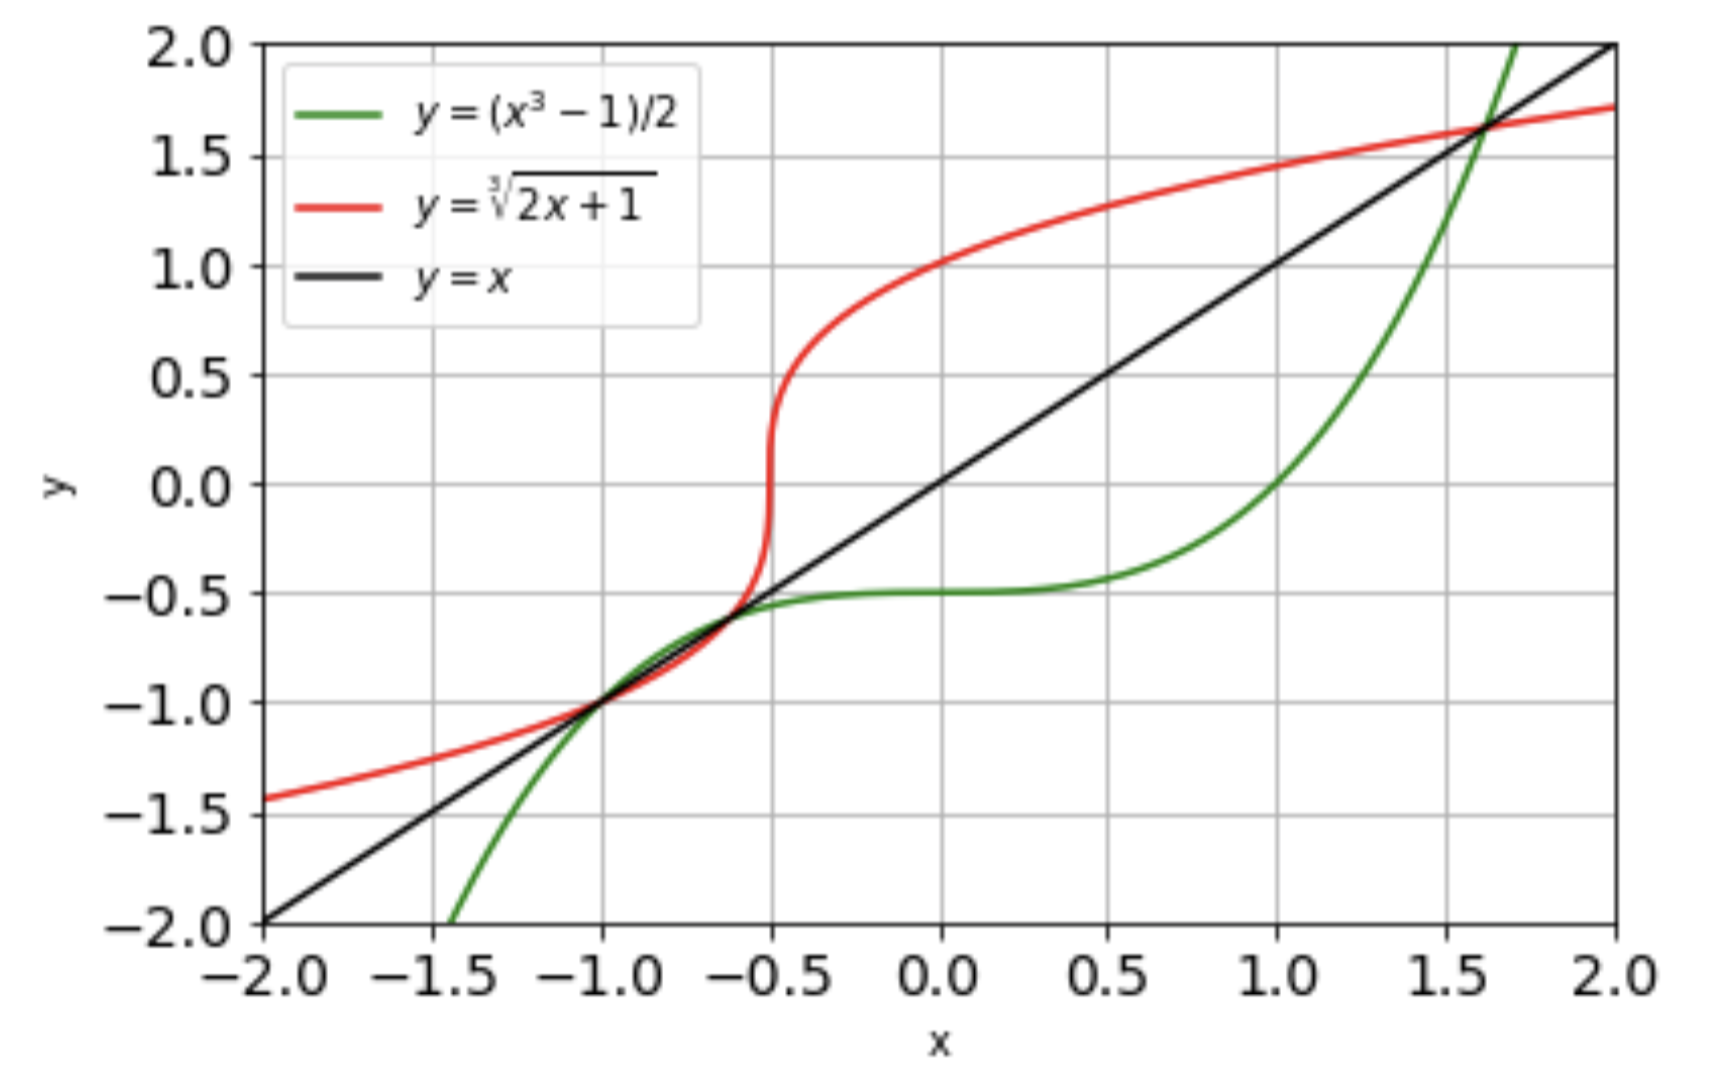
\includegraphics[width=10cm]{graph.jpg}
\end{center}


\vspace{33pt} 

{\Large 中間レポートおまけ問題.} (授業第1,2,5回の内容.)
\vspace{11pt}

次の問いに答えよ.

\vspace{11pt}

(1).
地球上ではいかなる時間でも, ある赤道上の点$x$とその対蹠点$y$で, $x$と$y$の気温が同じような点の組$(x,y)$が存在することを示せ.
ただし地球は球体であると仮定して良い.
ここで対蹠点とは地球の裏側の点のことである.
%\footnote{例えば杉本キャンパスは東経135度北緯34度に位置しているため, 杉本キャンパスの対蹠点は西経45度南緯34度である. 調べてみるとおそらくパラグアイの領海か排他的経済水域のように思われる. ちなみに杉本キャンパスの裏側はブラジルではない.}

\vspace{11pt}
 
(2). $a<b$なる任意の実数$a,b$について, $a<q<b$となる有理数$q$が存在することを示せ.

  \vspace{11pt}
 
\hspace{-11pt}{\Large $\bullet$ 中間レポートおまけ問題解答例.}

(1). 大きな実数$R>0$を取って, 地球の表面$S= \{ (x,y,z) | \sqrt{x^2 + y^2 + z^2} = R \}$として良い.
$$
\begin{array}{cccc}
F: &S& \rightarrow & \R  \\
&p& \longmapsto & \text{点$p$での気温}
\end{array}
\begin{array}{cccc}
\gamma: &[0,2\pi]& \rightarrow & S  \\
&\theta& \longmapsto & (R \cos \theta, R \sin \theta, 0)
\end{array}
$$
とおくと, 点$\gamma(\theta)$は地球$S$の赤道上の点であり,
$0 \leqq \theta \leqq \pi $について点$\gamma(\theta + \pi)$は点$\gamma(\theta )$の対蹠点である. そこで$[0,\pi]$上の関数$f$を

$$
\begin{array}{cccc}
f: &[0,\pi]& \rightarrow & \R  \\
&\theta& \longmapsto & F(\gamma(\theta + \pi)) - F(\gamma(\theta ))
\end{array}
$$
とすると, $f(\theta)$は連続であり\footnote{ここにある種の連続性を仮定している.}, 
$$f(\pi) = F(\gamma(2 \pi)) - F(\gamma(\pi ))
= F(\gamma(0)) - F(\gamma(\pi )) = - f(0) \text{である.}$$

$f(0)=f(\pi)$のとき, $f(0)=0$となる.
よって, $x=\gamma(0), y=\gamma(\pi)$とおけば, 
$y$は$x$の対蹠点であり, $F(x) = F(y)$から$x$と$y$の気温は等しい.

$f(0) \neq f(\pi)$のとき, $f(\pi) = -f(0)$であるので, 
$f(0) < 0 <f(\pi)$または$f(\pi) < 0 <f(0)$が成り立つ.
よって中間値の定理より, ある$c \in [0 , \pi]$があって$f(c)=0$となる.
以上より, $x=\gamma(c), y=\gamma(c+\pi)$とおけば, 
$y$は$x$の対蹠点であり, $F(x) = F(y)$から$x$と$y$の気温は等しい.

[補足]. その他面白い解答には部分点を与えました.

(2).
$c=\frac{a+b}{2}$とし, $\epsilon = \frac{b-a}{4}$とおく.
ある有理点列$\{ a_n\}$があって$\lim_{n \rightarrow +\infty} a_n =c$となる.
$\epsilon$-$\delta$論法から, ある自然数$N$があって
$N <n$ならば$|c - a_n| < \epsilon$となる.
よって$q=a_{N+1}$とおくと$q$は有理数であり
$$
c-\epsilon < q < c+ \epsilon
$$
である.
簡単な計算から$a<c-\epsilon $かつ$c+\epsilon <b$であるので, $a < q < b$である.

[補足]. アルキメデスの性質を用いた解答で, 証明に穴がない場合には, 正答としました.

 \vspace{33pt} 
   
   \hspace{-11pt}{\Large 中間レポートについて.}

第1問から第4問を通して, 正答率82\%でした. とてもよくできていたと思います.
各問題を通しての感想は以下のとおりです.
\begin{itemize}
\item [第1問.] 正答率82\%. 意外と計算ミスが多かったです. 特に(1)の計算ミスが非常に多かったです.
レポートを提出する前にはきちんと計算チェックをするようにしてください. また計算の過程を書いてない答案も見られました. きちんと計算の過程を書いてください. (減点の対象となる場合があります.)
\item [第2問.] 正答率71\%. おそらくベキ級数を使った適当な答案が出るだろうと思って出した問題です. しかしそういった答案は少ししかありませんでした. 補足でも述べた通り(1)は微分を5回やっても示せます.
\item [第3問.] 正答率98\%. ほぼ全員できてました. 非常に素晴らしいです. (4)の公式はマチンの公式と呼ばれます. 実は円周率$\pi$の近似値はマチンの公式に似た公式と$\Tan x$のテイラー展開を用いて求められています. 
\item [第4問.] 正答率70\%. 元々の問題は(2)だけでしたが, 流石にそれでは難しすぎると思い, (1)を加えました. 意外にも正答率が予想より高くてびっくりしました. 大変優秀だと思います.
\end{itemize}



%\vspace{11pt}

%(3). $\sqrt[3]{3}$の小数第10位までを求めるプログラムを作成せよ.ただし次の点に注意すること.\begin{enumerate}\item[注意1.] プログラミング言語に関しては自由だが, あまりにもマニアックな言語は控えてください.\footnote{Haskellは大丈夫です. 私はc, c++, pythonぐらいなら読めます.}\item[注意2.] \underline{この問題は$\sqrt[3]{3}$の値を求めるアルゴリズムを考える問題である.}そのため\text{print(pow(3,$\frac{1}{3}$))}という解答などは不正解とする.\item[注意3.] 処理時間があまりにも長い場合は不正解とする. 処理時間の目安は2秒とする.\item[注意4.] 提出方法に関してはgithub等にアップロードしてそのリンクをレポートに貼っても良いし, プログラムのソースファイルを(スクリーンショット等で)画像にしてその画像をそのままレポートに貼っても良いです. (メールやWebClassのダイレクトメッセージで, プログラムのソースファイルを直接私に送るなどでも良いです.) \\ \underline{この問題に限り, 提出方法は皆さんにお任せいたします. }
%目安として処理時間2秒程度とする.\end{enumerate}

%任意の点$(a,b)\in \R^2$と任意の正の数$r>0$について, 点$(a,b)$中心の半径$r$の円板を$$B =\{ (x,y) \in \R^2 : \sqrt{(x-a)^2 + (y-b)^2} \leqq r\} \text{\,\, とするとき, }$$  ある点$(c,d) \in B$があって, $c$も$d$も共に有理数である.
     
% \begin{flushright} {\LARGE 以上.}\end{flushright}


%$f(x,y)$を$C^1$級関数とし,$C^1$級変数変換を$(x(u,v),y(u,v)) = (u \cos v, u \sin v)$とする.$g(u,v) = f(x(u,v), y(u,v))$とする時, $\pdrv{g}{u}, \pdrv{g}{v}$を$\pdrv{f}{x},\pdrv{f}{y}$を用いてあらわせ.

%$f(x,y) = x^3 -y^3 -3x +12y$について極大点・極小点を持つ点があれば, その座標と極値を求めよ. またその極値が極小値か極大値のどちらであるか示せ.

 %$f(x,y,z)= xyz, g(x,y,z)=x+y+z-170$とする.$g(x,y,z)=0$のもとで$f$の最大値を求めよ.つまり$S : = \{ (x,y) \in \R^3: g(x,y,z)=0\}$とする時, $f$の$S$上での最大値を求めよ.ただし$f$が$S$上で最大値を持つことは認めて良い.
  
 %

 

\end{document}
